% Brief report style paper, which ended up being too long. Saved in its medium
% length format prior to an attempt to really shorten down the brief paper.

% It's about how a somatotopically ordered pattern can be
% re-established in the cortex based on information carried with
% thalamocortical axons afferent from the ventrobasal thalamus, but
% without specifying absolute positions as centre-points for the
% barrels. Everything in the paper should be tailored towards arguing
% this idea.

\documentclass[9pt,twocolumn,twoside,lineno]{pnas-new}
\templatetype{pnasresearcharticle}

%\title{Self-organization of whisker barrels in simulation requires competition between thalamocortical axons}
%\title{Simulated barrel cortex self-organizes using information carried by thalamocortical axons}
\title{Information carried by thalamocortical axons enables self-organization of the barrel field}
% While writing, don't stop for errors
%\nonstopmode


% Use letters for affiliations, numbers to show equal authorship (if applicable) and to indicate the corresponding author
\author[a,1]{Sebastian~S.~James}
\author[a]{Stuart~P.~Wilson}

\affil[a]{Department of Psychology, The University of Sheffield, Sheffield, United Kingdom.}

% $^{*}$Corresponding author email: Seb.James@Sheffield.ac.uk\vspace{1em}\\

% Please give the surname of the lead author for the running footer
\leadauthor{James}

% Please add a significance statement to explain the relevance of your work
\significancestatement{The mystacial whiskers of rodents are a complex,
  spatially ordered set of structures whose pattern is repeated in several
  locations in the brain. We contribute a self-organising mechanism by which
  the pattern can be recreated with minimal genetic pre-determination at each
  location; only two pairs of axon guidance gradients are required in each
  tissue. The pattern's togography is carried by the axons which grow from one
  tissue to another and interact variably (depending upon which whisker they
  are associated with) with the guidance gradients in the target tissue whilst
  competing with each other for space. We demonstrate that this mechanism
  recreates a realistic whisker barrel field and also accounts for the results
  of well-known gene misexpression experiments.}

\correspondingauthor{\textsuperscript{1}To whom correspondence should be addressed. E-mail: \href{mailto:seb.james@sheffield.ac.uk}{\nolinkurl{seb.james@sheffield.ac.uk}}}

% At least three keywords are required at submission. Please provide three to five keywords, separated by the pipe symbol.
\keywords{Barrel cortex $|$ Self-organization $|$ Somatotopy $|$ Center-point $|$ Pattern}

\begin{abstract}
Understanding how genetic information and spontaneous pattern formation
together give rise to the whisker barrels is an important challenge for
developmental neurobiology. The barrel patterning that coalesces in layer IV
has been described formally as a Voronoi tesselation, which is indicative of
an underlying developmental process based on local competitive
interactions. If pattern formation relies only on such intrinsic
self-organising processes, how can the somatotopic order at the periphery be
maintained in the projections from brainstem to thalamus and from thalamus to
cortex?
%
To investigate, we began by extending a existing computational model of axon
branching and synaptogenesis in thalamocortical projections under the
influence of molecular signalling gradients.  We found that, although these
processes alone are incapable of generating patterns of cortical fields that
are more intricate than the patterns already present in the signalling
gradients, the addition of competition between the branches of axons that
originate from different thalamic barreloids allowed a full barrel-field
pattern to emerge in the presence of only two gradients.
%
%However, a
%full barrel-field pattern emerges under the guidance of as few as four
%signalling gradients when the model is extended to introduce competition
%between the branches of axons that originate from different thalamic
%barreloids.
%
%We show that the key requirements for the emergence of realistic
%(Voronoi tesselation) patterning are i) at each cortical location
%thalamocortical projections compete for a limited number of available
%connections, ii) at each location the axonal branching rate of each
%thalamocortical projection is reduced by the total branching density of the
%other projections, and iii) the density of axon branching for each
%thalamocortical projection is conserved.
%
We demonstrate how a purely
self-organising system can initialise a pattern which can then be faithfully
replicated in multiple neural structures.
%We show that this minimal model of
%barrel self-organisation provides a parsimonious account of data from a range
%of classic studies in which intrinsic and extrinsic factors have been
%experimentally manipulated.
\end{abstract}

\dates{This manuscript was compiled on \today}
\doi{\url{www.pnas.org/cgi/doi/10.1073/pnas.XXXXXXXXXX}}

\begin{document}

% Blue for comments
\newcommand{\cmnt}[1]{\textcolor{blue}{#1}}
% Divergence symbol (Del dot Del)
\newcommand{\dvrg}{\nabla\vcdot\nabla}
% Emphasis shortcut
\newcommand{\e}{\emph}
% Bold shortcut
\newcommand{\bol}{\textbf}
% Math bold
\newcommand{\mb}[1]{\mathbf{#1}}
\makeatletter
\newcommand*\vcdot{\mathpalette\vcdot@{.35}}
\newcommand*\vcdot@[2]{\mathbin{\vcenter{\hbox{\scalebox{#2}{$\m@th#1\bullet$}}}}}
\makeatother

\maketitle
\thispagestyle{firststyle}
\ifthenelse{\boolean{shortarticle}}{\ifthenelse{\boolean{singlecolumn}}{\abscontentformatted}{\abscontent}}{}

\modulolinenumbers{}
\linenumbers

\dropcap{S}patial patterns in neural connectivity provide clues about the
constraints under which brains evolve and develop.
%Whether or not patterning
%governs information processing, models of the development of information
%processing circuits can be validated in terms of their ability to account for
%biological patterning \citep{purves_iterated_1992}.
%%see also \citealp{wilson_what_2015,bednar_cortical_2016}
One of the most
distinctive patterns of neural connectivity is found in the rodent
barrel cortex \cite{woolsey_structural_1970}.
%(\citealp{woolsey_pattern_1948,woolsey_structural_1970,welker_structure_1974},
%see \citealp{fox_barrel_2008}).
Understanding how this particular pattern forms might shed light on the
interplay of genetic and extrinsic factors that shape cortical circuits.
%, and on a wealth of
%anatomical, physiological, and behavioural data obtained using this
%model system.

The barrels are large cortical columns, identifiable from birth in layer 4 of
primary somatosensory cortex as dense clusters of thalamocortical axons, which
are enclosed by borders a few neurons thick from postnatal day 3
\citep{erzurumlu_development_2012}. In the plane tangential to the cortical
surface the barrels constitute a map of the arrangement of the whiskers on the
face,
%(see \citealp{yamakado_subdivision_1979})
such that the cells of adjacent barrels respond most strongly and most quickly
to deflection of adjacent whiskers \citep{armstrong-james_flow_1992}. The
barrels reflect subcortical whisker maps comprising cellular aggregates known
as barreloids in the thalamus \cite{van_der_loos_barreloids_1976} and
barrelettes in the brainstem.
%\citep{killackey_pattern_1980}.

%Each whisker and its corresponding barrelette, barreloid, and barrel can be
%identified by its position on a two-dimensional grid.
%\citep{zucker_coding_1969,killackey_pattern_1980,van_der_loos_barreloids_1976,haidarliu_size_2001}.
%
%The barrels are normally up to twice as long in the axis aligned to the grid
%‘rows’ compared to the ‘arcs’, and the rows are visible from day 2
%\citep{rebsam_refinement_2002} whereas the arcs become distinct by day 3
%\citep{erzurumlu_development_2012,rebsam_refinement_2002}.
%In metabotropic glutamate receptor 5 (mGlu5) knockouts the barrel rows develop
%but the arcs do not (\citealp{hannan_plc-1_2001} see also
%\citealp{fox_barrel_2008}), thus distinct processes likely guide development
%of the barrels with respect to the orthogonal grid axes.

Barrel formation requires afferent input, driven by whisker stimulation and by
thalamic calcium waves that propagate via mGlu5-receptor activation
\citep{anton-bolanos_prenatal_2019}.
%(\citealp{anton-bolanos_prenatal_2019}, see also
%\citealp{anton-bolanos_developmental_2018}).
Patterning also depends on a complex network of axon guidance processes, which
includes interactions between guidance molecules like ephrin-A5 and A7
\citep{miller_epha7-ephrin-a5_2006} and between adhesion molecules like
cadherin-6 and 8 \citep{bishop_regulation_2000}, and the
binding of p75 to neurotropins
\citep{bishop_distinct_2002}.
% or both citations?
%\citep{shimogori_fibroblast_2005,bishop_distinct_2002}.
%
%(\citealp{shimogori_fibroblast_2005,bishop_distinct_2002}
%; see also \citealp{dye_lifespan_2011,dye_lifespan_2011-1}).
This network is orchestrated by interactions between morphogens Fgf8 and Fgf17
and transcription factors Emx2, Pax6, Sp8, and Coup-tf1
\citep{shimogori_fibroblast_2005,bishop_regulation_2000}, which are expressed
in gradients that mark orthogonal axes and can be manipulated to cause the
barrels to stretch, shrink, shift, skew, and even duplicate \cite{assimacopoulos_fibroblast_2012}.
% A longer list of citations:
%\citep{shimogori_fibroblast_2005,assimacopoulos_fibroblast_2012,borello_sp8_2014,sahara_sp8_2007,ypsilanti_transcriptional_2016,sur_patterning_2005}.
%
While complex structure in protein expression can be observed for some genes,
such as the molecules Bhlhb5 \citep{joshi_bhlhb5_2008}, we are not aware of
any report of gene expression patterns with the complexity of the barrel field
and so the mechanism by which the barrels form seems likely to be one in which
the structure forms by self-organization.

The boundaries of the barrels form a Voronoi tesselation across the cortical
sheet \citep{senft_mouse_1991}. This patterning suggests that the barreloid
topology may be preserved in the initial projection of the thalamocortical
axons into the cortex, and that a barrel forms by the lateral branching of the
axons from their initial centres of mass, which ceases upon contact with the
axons branching from adjacent centres. According to this model the barrel
pattern could be entirely determined by the distribution of the initial centre
points, which would itself be determined by guidance cues. However, the
assumption of pre-arranged centres is difficult to resolve with the
observation that thalamocortical axons arrive in the cortical plate as an
undifferentiated bundle prior to barreloid formation within the thalamus
\cite{agmon_organized_1993}. % Plus erzurumli, probably

Alternatively, reaction-diffusion dynamics could generate a Voronoi-like
tesselation in the cortex without the need for pre-arranged centres, by
amplifying characteristic modes in the noisy initial distribution of bundled
axon branches, as a net effect of short-range cooperative and longer-range
competitive interactions between cells. According to this model the barrel
pattern would be determined by the relative strength of these interactions and
by the shape of the cortical field boundary. However, reaction-diffusion
dynamics alone are unlikely to be able to account for the precise
co-registration and topographic connectivity between emergent domains in
thalamus and cortex, the non-uniform sizes and spacing of the barrels to form
rows versus arcs, and the influence of gene expression gradients.

As theories of barrel patterning, the centre-point and reaction-diffusion
models are not mutually exclusive. Pre-organised centres in the initial
conditions could bias reaction-diffusion processes to generate the specific
somatotopic arrangement of barrels more reliably, and similarly the mechanisms
by which axons branch laterally from barrel centres may involve a tension
between cooperative and competitive interactions. However, a proof that barrel
patterning can in principle emerge within an undifferentiated bundle of
thalamocortical axons, based only on local interactions between cells, would
remove the need to invoke a global supervisor, i.e., to assume a separate
stage and/or extrinsic mechanism for pre-organising thalamocortical
connections.

We seek to establish whether it is possible for the observed arrangement of
barrels to self-organise in a system governed by reaction-diffusion dynamics,
under the guidance of molecular signalling gradients, and in the absence of
pre-defined centre-points.
%
Our approach is to represent in a computational model the minimal set of
biological assumptions that might lead to the emergence of barrel patterning
in simulation, and, if necessary, to add to this minimal set only assumptions
that can be represented by the local exchange of information between adjacent
cells. The emergence of barrel patterning under such conditions would serve as
an existence proof of the plausibility of the hypothesis that barrel
development is a self-organising process.

\section*{Models}

Karbowski \& Ermentrout \citep{karbowski_model_2004} developed a dynamical
model of cortical arealization capable of generating predictions about the
influence of signalling molecules on the size, shape, and topological
organization of emergent cortical fields. Their model describes competition
between thalamocortical projections for territory along an anterior-posterior
cortical axis. The equations of the model define how the density of
connections, $c(x,t)$, and the density of axon branches, $a(x,t)$, interact at time $t$
at each cortical location $x$, for $N$ thalamocortical projections indexed by
$i$.
%The Voronoi tesselation used to describe barrel patterning is a
%two-dimensional structure, hence we first extended the original model for
%simulation on a two-dimensional cortical sheet, and describe it here as such
%(i.e., substituting $x$ with the two-dimensional position vector $\mb{x}$ and
%substituting terms of the form $\frac{d}{dx}$ with the spatial gradient
%operator $\nabla$).
%
The model was derived from the assumption that the rates at which
thalamocortical synapses form and thalamocortical axons branch are
reciprocally coupled, resulting in expressions for the change in $c_i$ as a
function of $a_i$, and for the change in $a_i$ as a function of
$c_i$. Synaptogenesis is modelled [in two dimensions, so the variables are
$a_i(\mb{x},t)$ \& $c_i(\mb{x},t)$] as
%
\begin{equation} \label{eq:dc}
\frac{\partial c_i}{\partial t} =-\alpha c_i +\beta  \left(1 - \sum_{i'=1}^{N} c_{i'}\right)[a_i]^k.
\end{equation}
%
When the final term evaluates to zero, the density of thalamocortical
connections decays exponentially at a rate given by $\alpha$. This occurs when
the density of connections over all thalamic projections sums to one;
interpreted as a state in which all available cortical synaptic receptors are
occupied. Otherwise, the connection density is assumed to vary non-linearly
($k>1$) with the axon branching density.

Changes in axon branching density are assumed to depend also on the influence
of guidance molecules and on the density of branches at adjacent cortical
locations:
%
\begin{equation} \label{eq:da}
\frac{\partial a_i}{\partial t} = \nabla\vcdot\left(D \nabla a_i-a_i\sum_{j=1}^{M} \gamma_{i,j}\nabla \rho_j(\mb{x})\right) - \frac{\partial c_i}{\partial t} + \chi.
\end{equation}
%
The first term on the right describes the divergence (indicated by
$\nabla\vcdot$) of a quantity referred to as the `flux of axonal branching'
(the term enclosed by parentheses, called $\mb{J}_i(\mb{x},t)$).
%The central idea in heat diffusion
%models is that the change in temperature (over time) at a given location is
%proportional to the gradient in the temperature (over space) at that
%location. Substituting the branching density for heat, axons from a given
The flux consists of lateral diffusion across the cortical sheet at a rate
given by the diffusion constant $D$, and an interaction term, in which
branching is influenced by gradients in the concentration of $M$ distinct
molecular signals, $\rho(\mb{x})$. The influence of a given signal (indexed by
$j$) on a given thalamic projection (indexed by $i$), is determined by the
parameter $\gamma_{i,j}$ which may be positive or negative such that axons of
a given thalamic projection may branch preferentially towards either higher or
lower concentrations of each signalling molecule.
%Interactions for
%which this value is positive encourage axon branching in the direction in
%which the concentration of the signal is increasing, whereas negative
%interactions encourage branching in the opposite direction. Hence the axons of
%a given thalamic projection are assumed to branch towards either higher or
%lower concentrations of each signalling molecule.

The second term on the right of Eq.~\ref{eq:da} represents an assumption that the
axon branching density decreases when the number of connections being made
increases, and vice versa, i.e., that branches are required to form synaptic
connections. Note that we introduce the term $\chi=0$ here, so that we might
subsequently redefine $\chi$ to introduce competition between thalamic
projections.
%that we will show to be necessary for the emergence of a
%somatotopic pattern.

Two points are important to emphasise: First, notice that the only
difference between thalamic projections are the interaction strengths,
$\gamma_{i,j}$. Any differences between the size, shape, and location of
cortical fields that reliably emerge from the dynamics of the model must be
due to differences in the choice of these values only; Second, the formulation
of the model is at this point entirely local, in the sense that simulating the
dynamics requires no information to be communicated from cortical locations to
any but the immediately adjacent locations.

In addition to the choice of initial conditions (for the fields
$c(\mb{x},t=0)$ and $a(\mb{x},t=0)$) and the axon guidance fields
$\rho(\mb{x})$, the free parameters of the model are the number of
thalamocortical projections, $N$, constants $\alpha$, $\beta$, $k$, and $D$,
and the $N\times M$ interaction strengths, $\gamma$.

The dynamics of the model (Eqs.~\ref{eq:dc} \& \ref{eq:da}) were solved on a
hexagonal lattice of grid elements representing the cortical sheet, under the
assumption that axon branches cannot extend beyond the boundary of the sheet,
i.e., $\mb{J}_i(\mb{x},t) \big\rvert_{boundary} = 0$. We developed software
tools for imposing arbitrary boundary shapes on the lattice. The dynamics were
numerically integrated using fourth-order Runge-Kutta (with fixed time-step
${\delta}t$), and using Gauss's Theorem to compute the flux term.

\section*{Results}

\begin{figure*}
\begin{center}
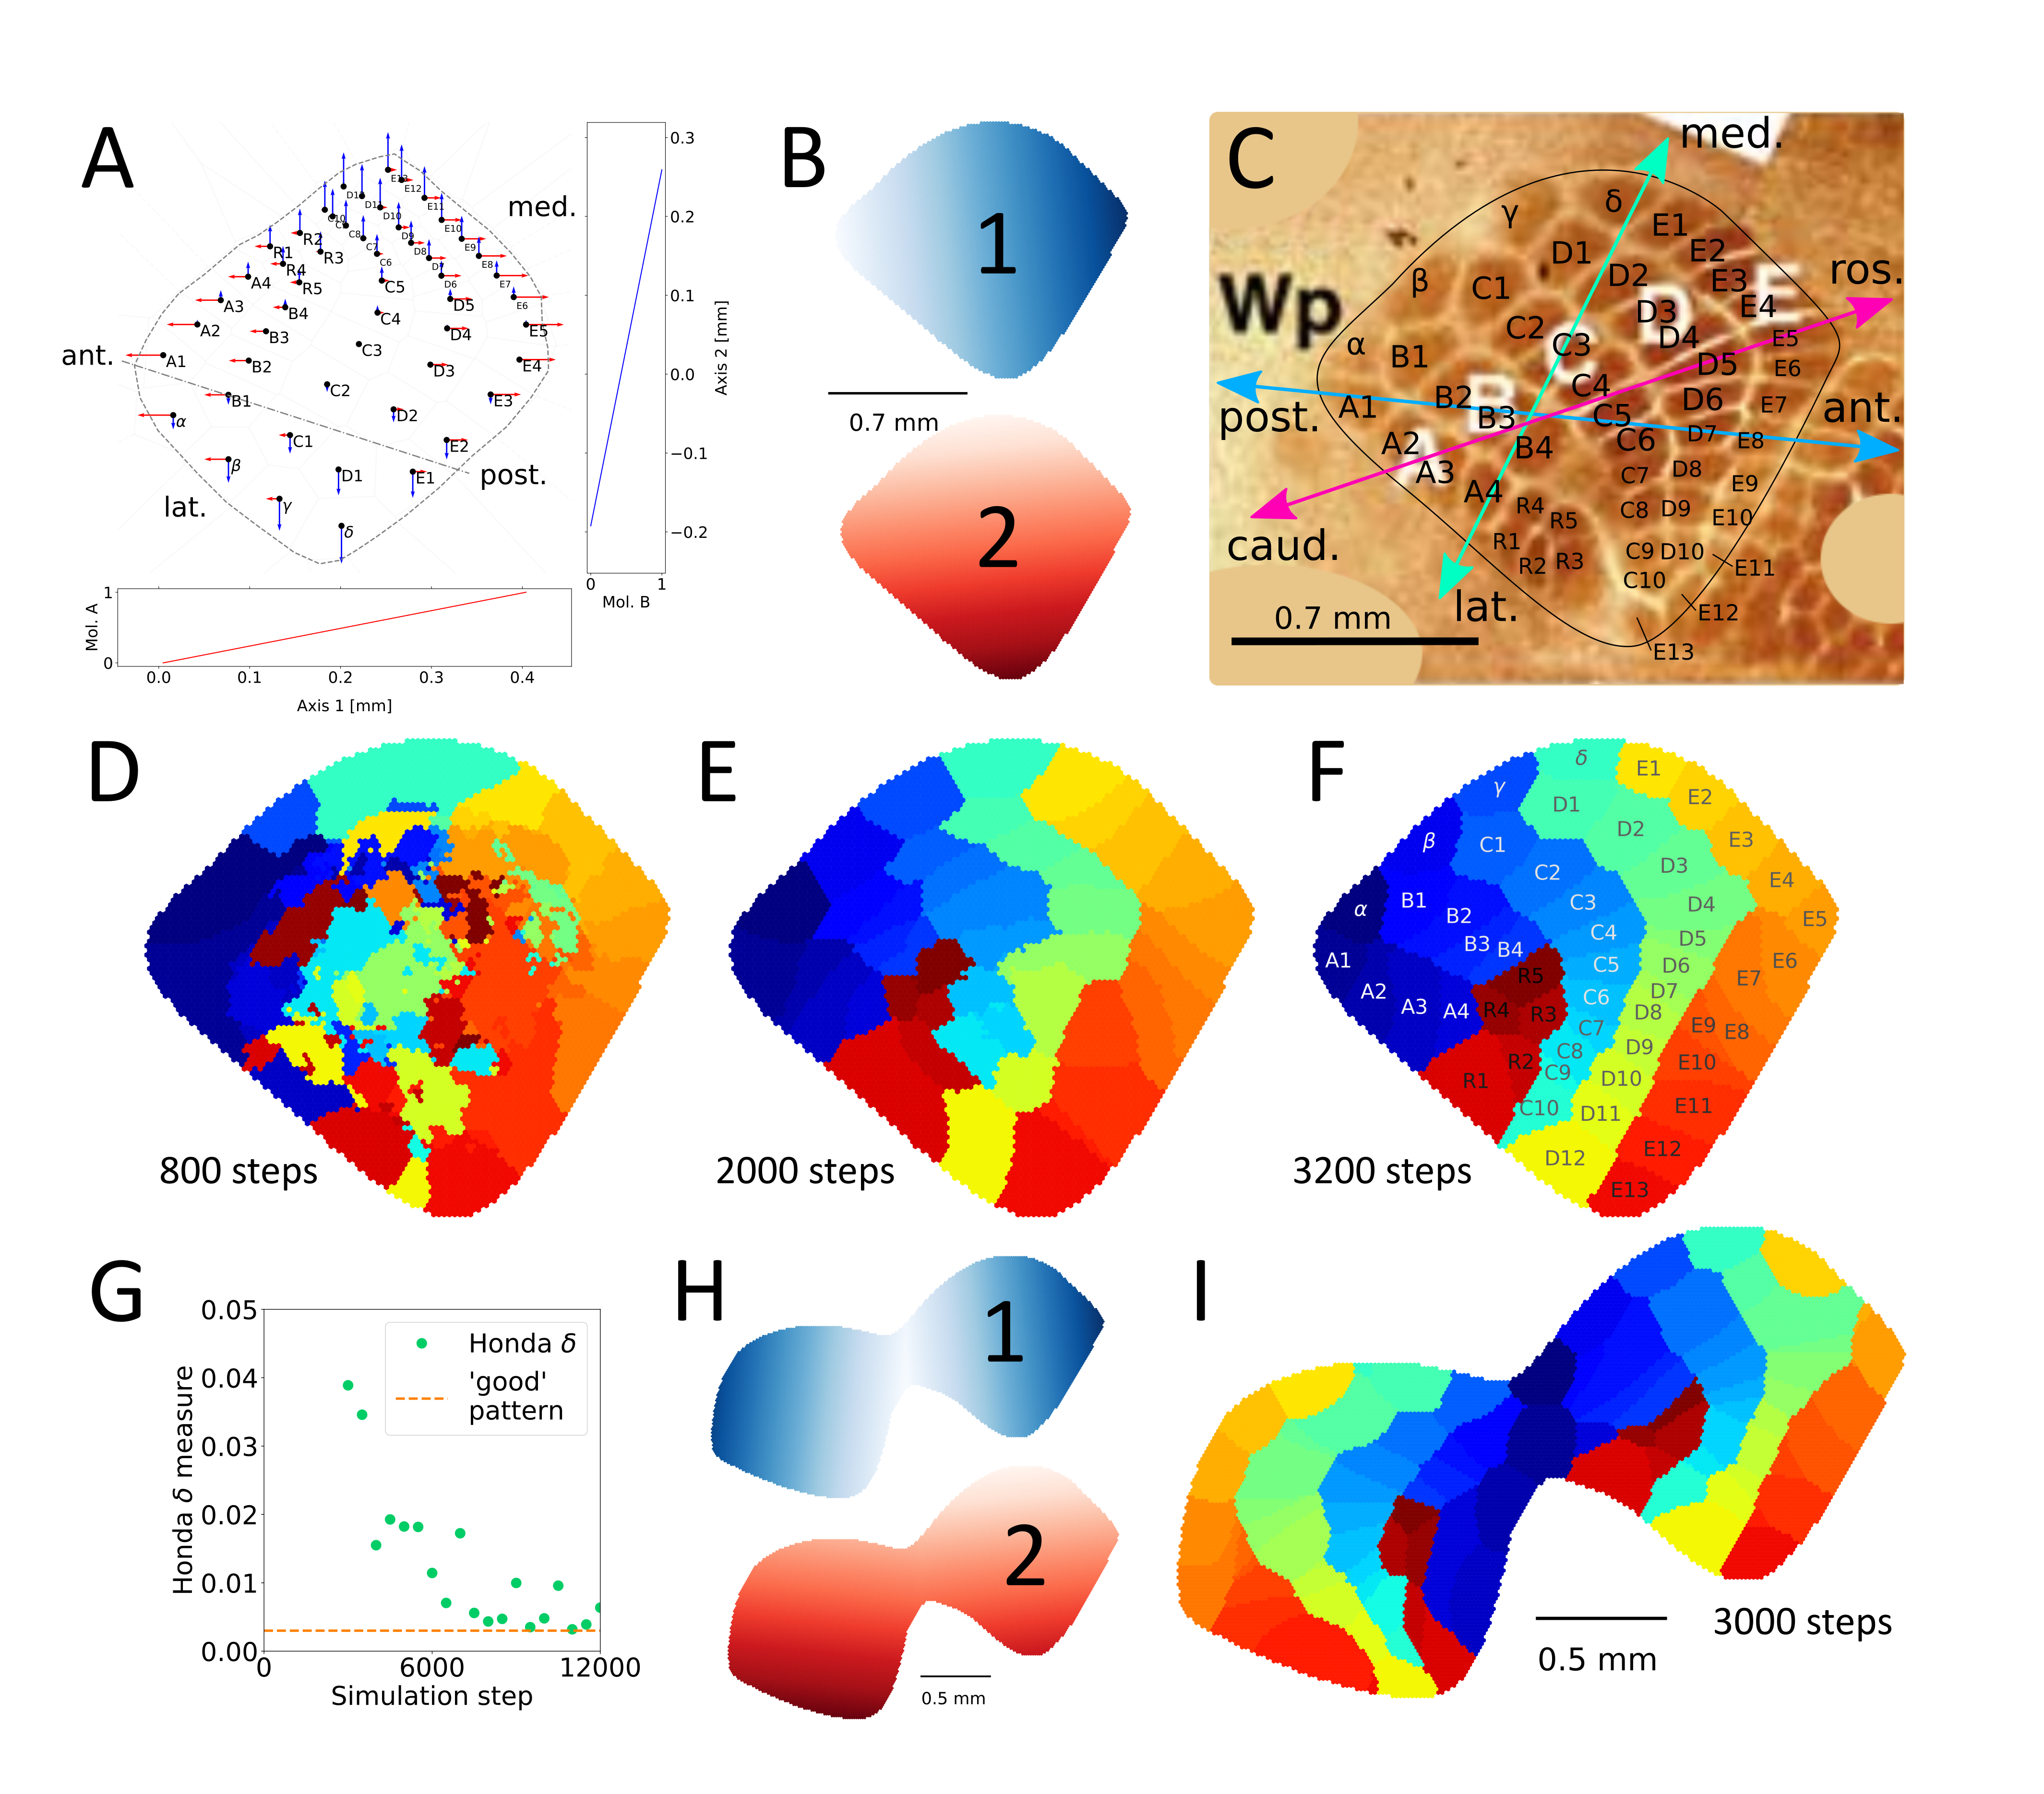
\includegraphics[width=\textwidth]{../briefpaper/MainFig.png}
\end{center}
%\vspace{-0em}
\caption{Simulated barrel fields. \textbf{A.} Barreloid centres taken from
  \cite{haidarliu_size_2001} are shown as black circles. Barreloids are
  labelled according to the usual convention. Labels R1 to R5 are the rhinal
  whisker barreloids. The dashed grey line represents the boundary of the
  barreloid field; the dot-dash line shows the anterior-posterior axis. It is
  assumed that there are two linearly increasing, orthogonal signalling
  gradients (molecules T1 \& T2) in the thalamus (side graphs), such that the
  location of each barreloid within the graded thalamic signal field can
  differentiate the efferent axons, with the result that axons from each
  barreloid interact to varying degrees with cortical signalling gradients
  (shown in panel B). Coloured arrows show, for each barreloid, the magnitude
  (and sign) of the interaction that its thalamocortical projection will have
  with the signalling gradients in the cortex. The mappings from barreloid
  location to interaction strength are linear. \textbf{B.} Guidance molecules
  in the simulated cortex. Molecule 1 is expressed high to low in an
  approximately anterior to posterior gradient. Molecule 2 is expressed
  lateral to medial (analogously to ephrin - Vanderhaegen et al) \textbf{C.}
  Whisker barrels from \cite{shimogori_fibroblast_2005}, with annotations for
  barrel identity and approximate axes.  \textbf{D-F.} Barrel cortex
  simulation. The maps indicate which thalomocortical axons make maximum
  connection density. Each hex element is coloured one of 52 unique colours
  depending on which e thalamocortical axon makes the most connections in that
  element. The mapping between barrel identity and colour is given in F.
  \textbf{G.} The Honda Voronoi measure as a function of simulation time for
  results shown in D--F. \textbf{H.}  Guidance molecules in the simulated Fgf8
  misexpression experiment. Molecule 1 is mirrored over the anterior-posterior
  axis \textbf{I.} The simulation indicates that the mirroring of the barrel
  field can occur as a result of the mirroring of guidance molecule 1 and the
  field boundary.}
\label{fig} % There's only one fig.
\end{figure*}

%\cmnt{If we need to present the results of the 2-D system with $\chi=0$, then
%  we'll do that first, showing a 2-D version of the simulation obtained by
%  running \code{james0 configs/karb.json}}

We first verified that the system given by Eqs.~\ref{eq:dc} \& \ref{eq:da}
described a two dimensional extension of the axon branching model in
\cite{karbowski_model_2004}. We showed that in the presence of three guidance
gradients varying only in one dimension (along the long axis of an elliptical
domain), five thalamocortical axon types, each interacting uniquely with the
three guidance gradients, would segregate into five separate regions. We
investigated a number of configurations of the guidance gradients, varying
their shape, $\rho(\mb{x})$, and number, $M$, and their effect on a varying
number of thalamocortical projections, $N$. In general, we were not able to
produce a complexity of structure in the resulting patterns of the
connections, $c(\mb{x},t\rightarrow\infty)$, which was not present in the
guidance patterns.


\subsection*{Branching competition is required to form somatotopically ordered barrels}

To investigate how the whisker barrel structure (Fig.~\ref{fig}C) might
form in the presence of only monotonically varying morphogen gradients, we
turned our attention to the competition for connections built into the
model. There \emph{does} exist an element of competition in the original model
(Eqs.~\ref{eq:dc} \& \ref{eq:da}). The term $\left(1 - \sum_{i=1}^{N}
c_i\right)$ in Eq.~\ref{eq:dc} ensures that once the available synaptic
receptors in a region have been fully occupied by one thalamocortical axon
type, there is no longer the possibility for other types to form
synapses. This competition turns out to be relatively weak, because it does
not strongly affect the branching density in that region; it is possible for
two or more TC axon types to have roughly equal branching density in some
region, leading to roughly equal numbers of connections forming for each TC
type, up until the `hard' connection limit is reached.

To introduce competition between the \emph{branching} of thalamocortical axon
types, we introduced the new term $\chi$ given by
%
\begin{equation} \label{eq:comp}
\chi(\mb{x}, t) = - \frac{\epsilon  a_i}{N-1} \sum_{i' \ne i}^{N} a_{i'}
\end{equation}
%
%with the choice $f(a) = a$,
which leads to a reduction in
%the rate of increase of branching density for axon type $i$
%$\frac{\partial a_i}{\partial t}$
${\partial a_i}/{\partial t}$
in regions where the branching density
of \emph{other} axon types is high. The new parameter $\epsilon$ governs the
strength of the branching competition and the factor $1/(N-1)$ ensures that the
strength scales with $N$.

With the addition of branching competition, it is necessary to introduce a
normalisation step, in order to prevent one TC type from out-competing every
other type. This represents the idea that for a fixed number of afferent
thalamocortical axons, the overall number of branches must have some upper
limit, given the finite resources available in each cell for building new
processes. We divisively normalize the branching density, dividing it at each
computational step by the mean branching density per unit area. It is then
multiplied by the branching density per unit area at time 0, which preserves
the effect of any disparity in the numbers of axons of each type which
innervate the cortical sub-plate:
%
\begin{equation} \label{eq:norm}
  a_i(\mathbf{x}, t) = \int_\Omega  a_i(\mathbf{x}, 0) d\sigma \; \frac {a'_i(\mathbf{x}, t)} {\int_\Omega
  a'_i(\mathbf{x}, t) d\sigma}
\end{equation}
%
The prime symbols indicate the use of the intermediate value of $a_i$ after it
has been computed according to Eqs.~\ref{eq:dc}--\ref{eq:comp} on the basis of
the system state at time $t-{\delta}t$. Integrals over $\Omega$ denote a
spatial integral over the domain of interest.

\subsection*{The model can transfer realistic barrel patterns}

With these changes we were able to generate grid-like patterns with
appropriate (linearly spaced) choices of the interaction parameters,
$\gamma$. To determine the $\gamma$ values suitable to recreate the cortical
barrel field by a principled method, we postulated that the interaction of
each thalamocortical axon growth cone with the ephrin gradients in the
cortical sub-plate might be determined by the location of the \emph{barreloid}
containing the axon's soma within signalling gradents \emph{in the
  thalamus}.
%That is, that interaction is grouped by barreloid identity.
%
%We therefore sought a map of the thalamic barreloids from the
%literature.
Ref.~\cite{haidarliu_size_2001} provided a comprehensive map of the
layout of the barreloids in rat, which is similar to mouse
\cite{van_der_loos_barreloids_1976}. We used these data to create the map of
52 barreloids shown in Fig.~\ref{fig}A. We postulated two linearly
varying molecules and used the barreloids' positions within this field to
generate the interaction parameters represented by the blue and red arrows.

We configured a simulation based on Eqs.~\ref{eq:dc}--\ref{eq:norm} to run on
a domain whose shape was matched to data from \cite{shimogori_fibroblast_2005}
(Fig.~\ref{fig}C). 52 separate axon branching fields were initialised with
random noise and given the $\gamma$ parameters from Fig.~\ref{fig}A. Two
orthogonal gradients were specified; molecule 1 with a posterior to anterior
gradient and molecule 2 with a medial-lateral gradient (resembling ephrin
A5). Fig.~\ref{fig}D--E shows snapshots of the connection density at
simulation times 0.08, 0.2 and 0.32 (${\delta}t=10^{-4}$), with colour
indicating the identity of the barreloid whose axons make maximum connections
at each location and \cmnt{contours showing where connection density passes
  0.5, indicating that each axon group is well localized}. A pattern emerges
which strongly resembles the barrel cortex in Fig.~\ref{fig}C, with `simulated
barrels' forming for whisker rows A to E, along with a suitably located group
for the rhinal whiskers.
%
Fig.~\ref{fig}G shows (using the Honda measure) that the simulated mechanism
does generate Voronoi patterns, in agreement with
\cite{senft_mouse_1991}.

% On stronger branching; not used in the results presented here.
% \cmnt{The realistic barrel pattern experiment is enhanced by stronger
%  branching competition:}
%
% To increase the strength of the competition, we choose an alternative form for
% $f(a)$ in Eq.~\ref{eq:comp} which has a geometric form for small $a$: $f(a) =
% \frac{1}{1 + e^{-m[a]^l}} - \frac{1}{2}$. The parameters $l$ and $m$ control
% the steepness and shape of the function.
%%% End of stronger branching competition %%%%%%%%%%%%%%%%%%%%%%%%%%%%%%%%%%%%

\subsection*{The barrel field reacts to changes in the expression pattern of guidance molecules}

A plausible theory of barrel patterning should reproduce the results of
experimental whisker barrel manipulations.
%
Here, we show that our mechanism reproduces the mirrored whisker barrel fields
reported in \cite{shimogori_fibroblast_2005,assimacopoulos_fibroblast_2012}
when an additional rostro-caudal source of Fgf8 is caused by
electroporation. We assume that a mechanism separate to ours governs the
definition of the boundary within which the barrel field will form and that
the additional Fgf8 source causes the boundary to become mirrored, with an
additional, posterior region forming. We also assume that under this
manipulation, the anteror-posterior guidance molecule (1) takes on a 'v'
shaped profile, with high expression at the far anterior and posterior of the
double barrel field domain, and low expression around the centre
(Fig.~\ref{fig}H). We assume molecule 2 is unchanged in its expression
pattern. Fig.~\ref{fig}I shows the pattern which forms with the simulation of
52 TC types having the same $\gamma$ parameters as set for the original
simulation (i.e.~from Fig.~\ref{fig}A). Similar, mirrored patterns form in
each side of the expanded domain. Note that for many of the 52 axon types, 2
fields form in spatially distinct locations (selected examples are shown),
though the straggler barrels $\alpha$ to $\delta$ and a few others (incl.~A1,
C1) appear in only single locations.

\section*{Discussion}

We set out to test the hypothesis that barrel patterning may emerge via
self-organising processes.
%
We first extended an existing model of neocortical arealization to simulate
pattern formation in two dimensions, inheriting from this model the assumption
that axonal branching and synaptogenesis are coupled, and that thalamic
projections compete for cortical territory under the influence of molecular
signalling gradients.
%
Realistic barrel patterning emerged only when terms were added to represent
the assumption that thalamocortical projections compete for a limited supply
of connections with cortical cells, that their branching rates are reduced by
the branching of other thalamocortical projections, and that the density of
axon branching is conserved for each projection.
%
The net effect of these local interactions is a Voronoi tesselation in which
localised clusters of thalamic projections become somatotopically organised on
the cortical sheet according to the relative values of coefficients specifying
the rates at which axons are attracted or repelled by orthogonal molecular
signal gradients.
%
According to this model, the pattern of barrels is determined by the
competitive and cooperative interactions between cells relative to the shape
of the cortical field boundary. By computing this simulation on a realistic
barrel field, we provide an existence proof that the somatotopic order of the
barrels can be transferred without the need for absolute positional
information on their centre-point locations. Instead, relative interaction
information, extracted from the source tissue of the afferent axons (the
thalamus) can reproduce the somatotopy regardless of changes to the boundary
shape or size. A similar process could enable the transfer of peripheral
pattern information (the ultimate source of the pattern?) to the barrelettes
in the brainstem and from the barrelettes to the ventro basal thalamus.

The requirement for two orthogonal guidance gradients is easy to understand;
this provides a coordinate system to differentiate locations within the
cortical sub-plate. It is interesting to note that in order to successfully
reproduce the barrel patterns of Fig.~\ref{fig}C, we found it necessary for
axon types to experience \emph{both} positive \emph{and} negative interactions
with the two gradients. If only positive interactions are permitted (that is
growth cones only move up the gradient) then the pattern is heavily skewed
towards one side of the domain.
%
If empirical data showed that only positive (or negative) interactions were
possible, then by having \emph{four} guidance gradients, as two, orthogonal,
opposing pairs, the same, balancing effect could be achieved. Such a pattern
of opposing pairs of expression gradients is known to exist in the cortical
transcription factors that are related to Fgf8.

% Can of worms?
We think of this process as taking place in the cortical sub-plate and have
reported that the pattern resembles a Voronoi diagram. Anatomical data
suggests that the somatotopy is determined within the sub-plate. However, the
actual barrel pattern forms in layer IV of the cortex, to which axons are seen
to rise, and so the final Voronoi layout of the barrels is likely to be
influenced by mechanisms taking place within layer IV. This may explain why,
as the Voronoi measure of the simulated barrel pattern improves, the
correspondence between the simulated, and measured barrel layout diverges.

% Anything to say about the misexpression experiment?

\subsection*{Supplementary Material}

The code and configuration required to reproduce the results in this paper are
available at \url{https://github.com/ABRG-Models/BarrelEmerge}.

\bibliography{../BarrelEmerge}

\end{document}
